\documentclass[12pt,a4paper,oneside,pdftex]{report}
\usepackage[utf8]{inputenc}
\usepackage[OT1]{fontenc}
\usepackage[finnish,english]{babel}
%\usepackage{colorprofiles}
%\usepackage[a-2b]{pdfx}

% Natbib allows you to select the format of the bibliography references.
% The first example uses numbered citations: 
\usepackage[square,sort&compress,numbers]{natbib}
% The second example uses author-year citations.
% If you use author-year citations, change the bibliography style (below); 
% acm style does not work with author-year citations.
% Also, you should use \citet (cite in text) when you wish to refer
% to the author directly (\citet{blaablaa} said blaa blaa), and 
% \citep when you wish to refer similarly than with numbered citations
% (It has been said that blaa blaa~\citep{blaablaa}).
% \usepackage[square]{natbib}

% The alltt package provides an all-teletype environment that acts
% like verbatim but you can use LaTeX commands in it. Uncomment if 
% you want to use this environment. 
% \usepackage{alltt}

% The eurosym package provides a euro symbol. Use with \euro{}
\usepackage{eurosym}
\usepackage{todonotes}

% Verbatim provides a standard teletype environment that renders
% the text exactly as written in the tex file. Useful for code
% snippets (although you can also use the listings package to get
% automatic code formatting). 
\usepackage{verbatim}

% The listing package provides automatic code formatting utilities
% so that you can copy-paste code examples and have them rendered
% nicely. See the package documentation for details.
% \usepackage{listings}

% The fancuvrb package provides fancier verbatim environments 
% (you can, for example, put borders around the verbatim text area
% and so on). See package for details.
% \usepackage{fancyvrb}

% Supertabular provides a tabular environment that can span multiple 
% pages. 
%\usepackage{supertabular}
% Longtable provides a tabular environment that can span multiple 
% pages. This is used in the example acronyms file. 
\usepackage{longtable}

% The fancyhdr package allows you to set your the page headers 
% manually, and allows you to add separator lines and so on. 
% Check the package documentation. 
% \usepackage{fancyhdr}

% Subfigure package allows you to use subfigures (i.e. many subfigures
% within one figure environment). These can have different labels and
% they are numbered automatically. Check the package documentation. 
\usepackage{subfigure}

% The titlesec package can be used to alter the look of the titles 
% of sections, chapters, and so on. This example uses the ``medium'' 
% package option which sets the titles to a medium size, making them
% a bit smaller than what is the default. You can fine-tune the 
% title fonts and sizes by using the package options. See the package
% documentation.
\usepackage[medium]{titlesec}
\usepackage{listings}

% The TikZ package allows you to create professional technical figures.
% The learning curve is quite steep, but it is definitely worth it if 
% you wish to have really good-looking technical figures. 
\usepackage{tikz}
% You also need to specify which TikZ libraries you use
\usetikzlibrary{positioning}
\usetikzlibrary{calc}
\usetikzlibrary{arrows}
\usetikzlibrary{decorations.pathmorphing,decorations.markings}
\usetikzlibrary{shapes}
\usetikzlibrary{patterns}


% The aalto-thesis package provides typesetting instructions for the
% standard master's thesis parts (abstracts, front page, and so on)
% Load this package second-to-last, just before the hyperref package.
% Options that you can use: 
%   mydraft - renders the thesis in draft mode. 
%             Do not use for the final version. 
%   doublenumbering - [optional] number the first pages of the thesis
%                     with roman numerals (i, ii, iii, ...); and start
%                     arabic numbering (1, 2, 3, ...) only on the 
%                     first page of the first chapter
\usepackage{aalto-thesis}
%\usepackage[mydraft,doublenumbering]{aalto-thesis}



% Hyperref
% ------------------------------------------------------------------
% Hyperref creates links from URLs, for references, and creates a
% TOC in the PDF file.
% This package must be the last one you include, because it has
% compatibility issues with many other packages and it fixes
% those issues when it is loaded.   
%\RequirePackage[pdftex]{hyperref}
\RequirePackage[pdfa]{hyperref}
% Setup hyperref so that links are clickable but do not look 
% different
\hypersetup{colorlinks=false,raiselinks=false,breaklinks=true}
\hypersetup{pdfborder={0 0 0}}
\hypersetup{bookmarksnumbered=true}
% The following line suggests the PDF reader that it should show the 
% first level of bookmarks opened in the hierarchical bookmark view. 
\hypersetup{bookmarksopen=true,bookmarksopenlevel=1}
% Hyperref can also set up the PDF metadata fields. These are
% set a bit later on, after the thesis setup.   


% Thesis setup
% ==================================================================
% If you do not find the command for a text that is shown in the cover page or
% in the abstract texts, check the aalto-thesis.sty file and locate the text
% from there. 
% All the texts are configured in language-specific blocks (lots of commands
% that look like this: \renewcommand{\ATCITY}{Espoo}.
% You can just fix the texts there. Just remember to check all the language
% variants you use (they are all there in the same place). 
% ------------------------------------------------------------------
\newcommand{\TITLE}{Working Agreements influence on software development productivity}
\newcommand{\DATE}{June 1, 2022}

\newcommand{\FTITLE}{Otsikko}
\newcommand{\FDATE}{Kesäkuu 1, 2022}

% Supervisors and instructors
% ------------------------------------------------------------------
% Usually thesis have one supervisor and one advisor. Sometimes you
% may have two advisors and, in double degree
% programs, you may have two supervisors. 
% If you have two supervisors, write both names here, separate them with a 
% double-backslash (see below for an example)
% Also remember to add the package option ``twosupervisors'' or
% ``twoinstructors'' to the aalto-thesis package (aalto-thesis.sty
% file line 72), so that the titles are in plural.

% Example of one supervisor:
\newcommand{\SUPERVISOR}{XXX Arto Hellas}
\newcommand{\FSUPERVISOR}{XXX Arto Hellas}

% If you have only one instructor, just write one name here
\newcommand{\INSTRUCTOR}{XXX Ari-Pekka Koponen}
\newcommand{\FINSTRUCTOR}{FM Ari-Pekka Koponen}

% Other stuff
% ------------------------------------------------------------------
\newcommand{\PROFESSORSHIP}{}
\newcommand{\FPROFESSORSHIP}{}
% Professorship code is the same in all languages
\newcommand{\PROFCODE}{}
\newcommand{\KEYWORDS}{}
\newcommand{\FKEYWORDS}{}
\newcommand{\LANGUAGE}{English}
\newcommand{\FLANGUAGE}{Englanti}

% Author is the same for all languages
\newcommand{\AUTHOR}{Petrus Holm}

% Currently the English versions are used for the PDF file metadata
% Set the PDF title
\hypersetup{pdftitle={\TITLE}}
% Set the PDF author
\hypersetup{pdfauthor={\AUTHOR}}
% Set the PDF keywords
\hypersetup{pdfkeywords={\KEYWORDS}}
% Set the PDF subject
\hypersetup{pdfsubject={Master's Thesis}}


% Layout settings
% ------------------------------------------------------------------

% When you write in English, you should use the standard LaTeX 
% paragraph formatting: paragraphs are indented, and there is no 
% space between paragraphs.
% When writing in Finnish, we often use no indentation in the
% beginning of the paragraph, and there is some space between the 
% paragraphs.

% Use this to control how much space there is between each line of text.
% 1 is normal (no extra space), 1.3 is about one-half more space, and
% 1.6 is about double line spacing.  
% \linespread{1} % This is the default
% \linespread{1.3}

% Bibliography style
% acm style gives you a basic reference style. It works only with numbered
% references.
\bibliographystyle{acm}
% Plainnat is a plain style that works with both numbered and name citations.
% \bibliographystyle{plainnat}


% Extra hyphenation settings
% ------------------------------------------------------------------
% You can list here all the files that are not hyphenated correctly.
% You can provide many \hyphenation commands and/or separate each word
% with a space inside a single command. Put hyphens in the places where
% a word can be hyphenated.
% Note that (by default) LaTeX will not hyphenate words that already
% have a hyphen in them (for example, if you write ``structure-modification 
% operation'', the word structure-modification will never be hyphenated).
% You need a special package to hyphenate those words.
\hyphenation{}

% added to remove error regarding comments / Pholm
\setlength {\marginparwidth }{2cm}

% The preamble ends here, and the document begins. 
% Place all formatting commands and such before this line.
% ------------------------------------------------------------------
\begin{document}
% This command adds a PDF bookmark to the cover page. You may leave
% it out if you don't like it...
\pdfbookmark[0]{Cover page}{bookmark.0.cover}
% This command is defined in aalto-thesis.sty. It controls the page 
% numbering based on whether the double-numbering option is specified
\startcoverpage

% Cover page
% These control in which language the cover-page information is shown
\pagenumbering{roman}
\coverpage{english}


% Abstracts
% ------------------------------------------------------------------
% Include an abstract in the language that the thesis is written in,
% and if your native language is Finnish or Swedish, one in that language.

%\input{0abstract.tex}


% Acknowledgements
% ------------------------------------------------------------------
% Select the language you use in your acknowledgements
\selectlanguage{english}

% Uncomment this line if you wish acknowledgements to appear in the 
% table of contents
%\addcontentsline{toc}{chapter}{Acknowledgements}

% The star means that the chapter isn't numbered and does not 
% show up in the TOC
\chapter*{Acknowledgements}



\vskip 10mm

\noindent 
\FDATE
\vskip 5mm
\noindent\AUTHOR

% Acronyms
% ------------------------------------------------------------------
% Use \cleardoublepage so that IF two-sided printing is used 
% (which is not often for masters theses), then the pages will still
% start correctly on the right-hand side.
\cleardoublepage
% Example acronyms are placed in a separate file, acronyms.tex
%\addcontentsline{toc}{chapter}{Abbreviations and Acronyms}
\chapter*{Abbreviations and Acronyms}

\noindent
\begin{longtable}{@{}p{0.25\textwidth}p{0.7\textwidth}@{}}
CD & Continuous Delivery \\
CI & Continuous Integration \\
DORA & DevOps Research and Assessment \\
IEEE & Institute of Electrical and Electronics Engineers \\
IPCT & In Progress Cycle Time \\
IRCT & In Review Cycle Time \\
PR & Pull Request \\
PRCT & Pull Request Cycle Time \\
RMCT & Ready to Merge Cycle Time \\
SDLC & Software Development Life Cycle \\
WA & Working Agreement \\
WIP & Work In Progress \\
\end{longtable}

% Table of contents
% ------------------------------------------------------------------
\cleardoublepage
% This command adds a PDF bookmark that links to the contents.
% You can use \addcontentsline{} as well, but that also adds contents
% entry to the table of contents, which is kind of redundant.
% The text ``Contents'' is shown in the PDF bookmark. 
\pdfbookmark[0]{Contents}{bookmark.0.contents}
\tableofcontents

% List of tables
% ------------------------------------------------------------------
% You only need a list of tables for your thesis if you have very 
% many tables. If you do, uncomment the following two lines.
% \cleardoublepage
% \listoftables

% Table of figures
% ------------------------------------------------------------------
% You only need a list of figures for your thesis if you have very 
% many figures. If you do, uncomment the following two lines.
% \cleardoublepage
% \listoffigures

% The following label is used for counting the prelude pages
\label{pages-prelude}
\cleardoublepage

%%%%%%%%%%%%%%%%% The main content starts here %%%%%%%%%%%%%%%%%%%%%
% ------------------------------------------------------------------
% This command is defined in aalto-thesis.sty. It controls the page 
% numbering based on whether the double-numbering option is specified
\startfirstchapter
\pagenumbering{arabic}

% Add headings to pages (the chapter title is shown)
\pagestyle{headings}


% The contents of the thesis are separated to their own files.
% Edit the content in these files, rename them as necessary.
% ------------------------------------------------------------------


\chapter{Introduction - 2s}

\todo[inline]{motivation}
\todo[inline]{swarmia}
\todo[inline]{working agreements}

\section{Problem statement}

\todo[inline]{zero hypothesis: WAs have no effect on CT}

\begin{enumerate}
    \item[{\bf RQ1}] How do teams use Working Agreements?
    \item[{\bf RQ2}] How do Working Agreements influence team productivity?
\end{enumerate}

For RQ1, we examine the usage data of Swarmia teams. The aim is to find out how popular is the Working Agreements feature and how teams have configured it. 

We look into RQ2 from two aspects: Do Working Agreements overall influence team productivity and if they do, are some configurations of working agreements more influential than others. 

\section{Scope and Methodology}

\section{Results}

\section{Structure}


\chapter{Background}

\section{Software engineering}

The craft of software engineering emerged during the 1960s. Software crisis, the growing gap between expectations and results for software, called for a more systematic approach to software production~\cite{naur_peter_software_1969}. Authors suggested that software should be considered a branch of engineering, like hardware. NATO-organized conference in 1968 widely launched the new, engineering-inspired approach to software production.

Even though the comparison to engineering was initially used to provoke thought~\cite{naur_peter_software_1969}, it has since become a part of the software production vocabulary. However, the concept of software engineering has remained a topic of dispute in academia. \citet{boehm_software_1979} leans to the Webster dictionary definitions for software and engineering, combining them to a formal definition of software engineering: applying science to create "useful to man" computer programs and documentation. He argues that the difference between arbitrary development and software engineering is that the latter ensures the result is useful for the end-users, satisfying the specification. On the other hand, Sommerville establishes the gap between software development and software engineering: he defines software development as the actual development process where code is written, whereas software engineering is tied to the life cycle of the software – from planning to maintenance.~\cite{sommerville_software_2016}

The engineering mindset and the lifecycle of the software are included in IEEE's take on software engineering. The definition can be described as combining Boehm's and Sommerville's definitions. For this thesis, we will be using the IEEE definition.~\cite{ieee_ieee_1990}

Software engineering can be divided into four main activities: software specification, development, validation, and evolution.~\cite{sommerville_software_2016} These steps can also be called a software process or a software development life cycle (SDLC). Commonly used SDLCs include the Waterfall model, Validation \& Verification model (V model), and Agile methods.~\cite{balaji_waterfall_2012} Projects can benefit from different approaches: dimensions such as level of risk, budget, or project timeline vary between the SDLCs.~\cite{alshamrani_comparison_2015, cohen_introduction_2004} The industry data shows a trend towards the iterative approaches~\cite{sommerville_software_2016}. 

\subsection{Waterfall model}

The so-called Waterfall model is widely referred to as the most well-known SDLC. Waterfall model consists of 5 sequential process stages: requirements analysis, design, coding, testing, and maintenance.~\cite{alshamrani_comparison_2015} As the name implies, a project following the Waterfall model is one-way: it moves only forwards, and the different stages do not overlap. Each stage produces a deliverable to be used as a basis for the upcoming stage~\cite{balaji_waterfall_2012}. 

In practice, projects rarely blindly follow the Waterfall model: upcoming stages are prepared parallel to the current one, and previous stages are revisited when the need arises.~\cite{sommerville_software_2016} This "iterative Waterfall" is in line with the original model from the research paper Waterfall is derived from: the author originally intended the method to be used in an iterative manner~\cite{royce_managing_1987}.

A major shortcoming of the Waterfall model is that the software is delivered only once. On the other hand, it is good if the requirements are well-known beforehand and stay relatively static during the project. For example, a security system for a power plant would be a potential use case for the method.

\subsection{Agile methods}

Agile methods is an umbrella term that includes methodologies like Extreme Programming~\cite{wells_don_extreme_2018}, Lean Development, and Scrum~\cite{scrumorg_home_2022}. The terminology is further complicated due to the improper usage of the term in the industry. The common properties of Agile methods include iterative development, focus on communication, and a critical stance toward intermediate deliverables like requirements. Furthermore, Agile evangelists have agreed that Agile is more about a "state of mind" rather than a single process or methodology.~\cite{cohen_introduction_2004}

In iterative development, new versions of a working product are delivered constantly: most productive teams deploy software to production even multiple times in a day~\cite{forsgren_accelerate_2018}. This approach enables the end-users to use the software from the early days of the development cycle. Development teams can receive constant feedback from users and iterate the software accordingly for the next releases.~\cite{balaji_waterfall_2012}

Focus on communication encourages development teams to enable low-threshold, constant communication practices instead of documentation-heavy decision-making methods. Agile methods introduce practices like daily stand-up meetings and pair programming to support this~\cite{fowler_agile_2001}. When Agile methods emerged, co-locating team members were also seen as the key to success for working communication~\cite{cohen_introduction_2004}. With the possibilities presented by modern collaboration platforms like Slack and Zoom, low threshold communication has become possible for remote teams – working from the same physical location is no longer seen as crucial for Agile implementation.

Another definitive characteristic of Agile methods is the critical stance toward intermediate, non-critical deliverables. By reducing the resources spent on these artifacts, teams can focus their efforts on developing the product.~\cite{cohen_introduction_2004} The self-managing nature of Agile teams further promotes the idea that they have the best context to prioritize and plan their work.~\cite{alshamrani_comparison_2015} 

Even though Agile has an evergrowing status in the software development world, traditional methods like Waterfall are still needed. Large teams and complex projects are seen as environments where more structured processes should be preferred. On the other hand, teams are increasingly incorporating Agile properties into their traditional software processes and vice versa.~\cite{cohen_introduction_2004} 

\subsection{DevOps}

Agile has transformed the way software is developed. However, in the software lifecycle, the performance of testing, deployment, and post-deployment functions like fault recovery should be considered. DevOps brings development and IT operations closer together, bridging the gap between these silos and enabling responsiveness throughout the lifecycle of the software~\cite{hemon-hildgen_agile_2020}. DevOps aims to shorten the software development lifecycle by introducing automated tools that ship code to production faster, boosting both productivity and quality of development\cite{cois_modern_2014}. According to~\citet{humble_why_2011}, DevOps practices can be divided into four main aspects: automation, culture, sharing, and measurement. 

The most distinctive automation practices introduced by DevOps are continuous integration (CI) and continuous delivery (CD). In continuous integration, the developers' changes are often submitted back to the main branch as soon as possible, usually preceded by a build task and automated unit tests run by a CI worker. CI is often followed by CD, which is in charge of integration testing, end-to-end testing, and finally, deploying the approved version into a staging environment. The abbreviation "CD" is commonly also used to refer to continuous deployment. 

In addition to the steps in continuous delivery, continuous deployment automates software deployment to production environments. In contrast, continuous delivery pipelines require the user's manual interaction to initialize deployments. In the industry, CD usually refers to continuous delivery, though the term is used in quite a liberal manner. Systems consisting of both CI and CD functions are called the CI/CD pipeline. In modern-day DevOps, a stable CI/CD pipeline is the backbone of the team's success: In addition to customer satisfaction, implementing these practices can have an organizational impact, such as improved work satisfaction \cite{forsgren_accelerate_2018}. 
 
In essence, DevOps is about ways of working. Sociotechnical factors must be considered to create a well-functioning DevOps function~\cite{hemon-hildgen_agile_2020}. Implementing DevOps requires changes to the organization's work culture and a change of mindset from individual contributors. For example, rotating responsibilities and increased information sharing are ways to enforce DevOps practices.~\cite{lassenius_agile_2015}

Measuring processes is a cornerstone of increasing efficiency. In DevOps, production environments are measured continuously, and these metrics are used as gauges of development productivity~\cite{lassenius_agile_2015}. An increasing trend is also to measure the development processes directly: For example, statistics from version control systems are analyzed to extract information on the organization's health~\cite{forsgren_accelerate_2018}.

\section{Developer productivity}

\subsection{Productivity in general}
Productivity in industrial engineering is defined as the ratio of input and output\cite{syverson_what_2011, chew_no-nonsense_1988}. In manufacturing, input and output are relatively easily measured as the used resources and the produced goods. On the other hand, non-manufacturing businesses rely on more complex definitions: in knowledge work, person-hour is not considered a relevant metric of productivity~\cite{tangen_demystifying_2005}. The definition of output has also been under debate. In 1988, Chew proposed that output should include metrics other than "the number of units," for example, quality, timeliness, and price of the product~\cite{chew_no-nonsense_1988}. Many relatively similar context definitions have also emerged in the literature~\cite{tangen_demystifying_2005}.

The terms productivity and performance are sometimes used interchangeably. To further complicate the terminology, the authors define performance as a component of productivity and vice versa. Based on a vast amount of literature research, Tangen defines performance as an "umbrella term of excellence" consisting of productivity and other non-cost elements. In contrast, productivity is defined as a "physical phenomenon" – the ratio of input and output~\cite{tangen_demystifying_2005}. As an example of the opposite approach, SPACE authors define performance as the "outcome of a system or process," measured by metrics like service health or customer satisfaction. Productivity in the SPACE framework is about the sum of its parts, with performance as one of them~\cite{forsgren_space_2021}. To sum things up, these terms are used to refer to varying phenomena in different situations.

In the examples before, productivity is reviewed from the company's perspective. Often it is beneficial to look into the metrics of a smaller entity: a department, a team, or an individual~\cite{forsgren_space_2021, tangen_demystifying_2005}. These metrics can provide more accurate insights into the entity in question.

When measuring the productivity of teams or individual employees, it can be tempting to incentivize them based on the metrics. For example, software developers could get promotions or raise if they contribute more than average to the product. Often these ambitions can lead to unwanted results as employees optimize their work to meet the metric rather than focusing on the company's interests~\cite{symons_software_2010, chew_no-nonsense_1988}. For example, if the metric used was the number of pull requests, it would be tempting to break the work into tiny increments to pump up the numbers. Individual preferences further tricky the topic, as some employees by habit contribute more commits than others~\cite{oliveira_code_2020}. 

\subsection{Productivity in software engineering}
Determining the productivity of engineers is seen as crucial for the success of software development. Therefore, substantial research has been conducted in the past years.\cite{oliveira_code_2020} No consensus has been found on measuring productivity accurately. Historically, source code-based metrics such as lines of code or amount of commits have been utilized~\cite{oliveira_code_2020}. Nowadays, these metrics are considered, at best, an incomplete representation of the true productivity~\cite{forsgren_space_2021}.

Modern frameworks have explored the work of a software engineering team as a joint effort: as popular SDLCs emphasized teamwork, productivity should be assessed in the same context. The team is seen as the "basic work unit"~\cite{moe_overcoming_2010}, and the research has shifted towards how teams can improve together. Even though high-performing individuals are still seen as a valuable asset, companies should focus on building and enabling high-performing teams~\cite{forsgren_space_2021}. 

Agile methods estimate productivity by estimating velocity – units of completed work in a time frame. Although velocity is considered a better indicator of productivity than source code metrics, it has significant drawbacks. The topic is widely covered by \citet{forsgren_accelerate_2018} in their industry-shaping book \textit{Accelerate: The Science of Lean Software and DevOps: Building and Scaling High Performing Technology Organizations}. Most importantly, velocity is highly relative to the context and should not be used as an absolute metric. Secondly, velocity is an excellent example of a metric prone to be gamed by the employees, as described previously.~\cite{forsgren_accelerate_2018}
 
\subsection{Developer productivity frameworks}

Partly due to the misconceptions about developer productivity, research has gravitated towards finding reliable ways to discuss, measure, and enhance developer productivity. DevOps Research and Assessment (DORA), an Alphabet Inc subsidiary, has pioneered the research of DevOps and developer productivity. In their book Accelerate, they present four key metrics to measure software delivery performance, often referred to as the DORA metrics. The metrics are as follows: 

\begin{enumerate}
\item Lead Time
\item Deployment Frequency
\item Mean Time to Restore
\item Change Fail Percentage
\end{enumerate}

Lead Time is a metric derived from Lean manufacturing to the software context. It refers to the time from a feature request to the change that fulfills the request. Often in software, the changes are not directly requested by single customers but instead decided by the teams using large amount of input from stakeholders. DORA metrics define Lead Time as the time from the first commit to code running in the production environment~\cite{forsgren_accelerate_2018}.

In this thesis, we use Lead Time to refer to the time from the first commit to a new branch to the moment it is merged to the main branch, as seen in figure \ref{fig:CycleTime}. The industry term for this metric is Pull Request Cycle Time. 

\begin{figure}[ht]
    \begin{center}
        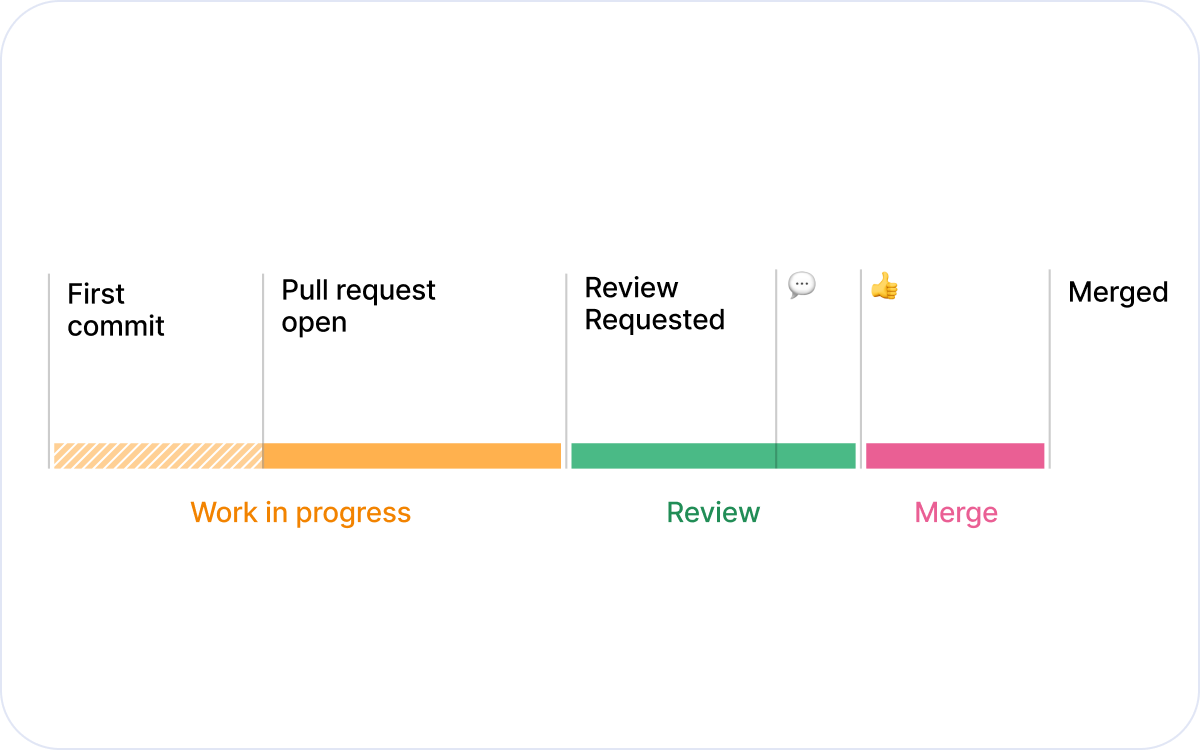
\includegraphics[width=13.5cm]{images/cycletime-defined}
        \caption{Pull Request lifecycle~\cite{swarmia_reducing_2022}}
        \label{fig:CycleTime}
    \end{center}
\end{figure}

Batch size has been popularized by it's use as a key performance metric in the Toyota Production System~\cite{ono_toyota_1988}. DORA researchers note that batch size is a sub-optimal metric in the software development context. Therefore, they chose Deployment Frequency as a suitable proxy to estimate the batch size. Deployment Frequency is the frequency of pushing a new version to the production environment.  

Lead Time and Deployment Frequency are metrics for software delivery tempo. Two additional metrics are used to determine if the increase in tempo has disadvantages in terms of software quality or system stability: Mean Time to Restore and Change Fail Percentage. Both of these measure situations where the production environment has failed. The authors articulate that failure is a common situation in rapidly changing software systems, and the absolute amount of failures is an obsolete metric. Instead, they propose two better suitable metrics: the time used to restore an application after an incident and the percentage of changes that lead to a production system failure. 

In Accelerate, the results are precise: increasing software delivery tempo has no negative impact on stability or quality. Instead, teams that performed well in the first two metrics also had better results in the rest measures. 

A more recent work from the DORA team is called the SPACE framework. The framework is named after its dimensions: satisfaction and well-being; performance; activity; communication and collaboration; and efficiency and flow. The framework extends DORA metrics by including, for example, perceived metrics. 

The researchers argue that productivity measurement should not rely on a single metric but rather include at least three metrics from the SPACE dimensions. Furthermore, the metrics should include quantitative, qualitative, and individual and team-level metrics. Also, performance measures on the organizational level are critical to getting a comprehensive image of productivity. 

The SPACE publication proposes a set of example metrics to concretize the framework. These proposals are not to be used as is but rather serve as an inspiration for those developing productivity tracking systems.~\cite{forsgren_space_2021}

\section{Software engineering as teamwork}

Work is often organized around teams. To distinguish a team from other groups that work together, we use the definition by Katzenbach \& Smith: "a team is a small number of people with complementary skills who are committed to a common purpose, set of performance goals, and approach for which they hold themselves accountable"~\cite{katzenbach_discipline_1993}. The fundamental difference is the accountability on both individual and team levels: team members are primarily responsible for each other, their supervisors, or other stakeholders~\cite{katzenbach_discipline_1993}.

In software engineering, teams work together to design, develop and maintain products. Working as a team offers upsides such as increased employee satisfaction, innovation, and productivity~\cite{moe_teamwork_2010}. In modern software development, the team is considered as the basic work unit rather than the individual contributor~\cite{moe_overcoming_2010}. This shift has motivated companies and executives to focus on building hyper-performing teams.

\subsection{Self-managing teams}

Modern software development methods encourage, or even insist on, the use of self-mana\-ging teams~\cite{moe_teamwork_2010,fowler_agile_2001}. Other terms used to define the phenomena include self-organizing team, autonomous team, and empowered team. Even though most studies report that forming self-managing teams leads to positive outcomes, there have also been opposing conclusions. Factors like poor leadership or the broader nature of the situation can lead to the difficulty of implementing such a team~\cite{moe_teamwork_2010}. 

To enable genuine self-management within a team, company leadership and other internal stakeholders must respect the team's independence and improvement efforts~\cite{moe_overcoming_2010}. Additionally, teams are not usually designated with a leader: instead, they are expected to form processes for a shared leadership function. Even though shared leadership can lead to better functioning teams, it adds more complexity and requires better cohesion and communication.~\cite{solansky_leadership_2008}

To improve, self-managing teams have to change their behavior, either by self-managing or from an external stimulus. Teams that can self-improve can achieve more autonomy than their counterparts. Norms, standards that regulate team members' behavior, are of the essence when building a productive software development team~\cite{abrahamsson_exploring_2016}. Norms can include technical and non-technical rules; for example, teams can commit to test-driven development or promote pair programming. The impact of norms for development teams is achieved through increased simplicity of standard processes: team members can trust that their colleagues do certain activities and refrain from the unwanted ones~\cite{abrahamsson_exploring_2016}. 

Team norms can be formed in two ways: organically within the team or by others, or as part of the organization's guidelines or direct influence~\cite{teh_social_2012}. Agile teams tune their ways of working during sprint retrospective meetings. Teams can also host dedicated sessions to discuss their norms: many SDLCs encourage teams to review their methods regularly. To enforce the norms, teams use whiteboards, notifications, and other reminders to refresh their memory and keep each other accountable.  

\subsection{Tools for teamwork}

Teams use a large number of tools to facilitate their work. Issue trackers like Jira, version control systems like Git, and chat tools like Slack play a central role in the day-to-day interaction of software development teams. Many team norms revolve around how team members are expected to use these applications. For example, the developers could commit to preferring public channels over direct messages in an instant messaging program.

 As a large part of information-intensive work is done using IT systems, there lies a remarkable efficiency improvement potential in these tools. Teams can aim to boost their performance with the help of software. For example, using web-based spreadsheet editor can reduce the need for manually sharing new versions within the team.

In addition to systems designed to help teams work together, there exists software solutions to improve team performance. Especially in software development, where the team's outputs are mainly lines of code, it is a tempting idea to conduct team performance metrics from the codebase~\cite{mcintosh_empirical_2016}. Authors argue that these kind of tools are problematic, as they only focus on outputs, reduce quality out of the equation and in essence, provide a one-sided view on the team's health~\cite{forsgren_space_2021, forsgren_accelerate_2018, oliveira_code_2020}.

To tackle this dilemma, a new wave of solutions addressing team performance has emerged. The tools are openly opinionated and aim to influence their client companies to use specific popular development methodologies, such as Continuous Integration. Examples of such tools include LinearB~\cite{linearb_developer_2022}, Haystack~\cite{haystack_haystack_2022}, Jellyfish~\cite{jellyfish_align_2022}, and Swarmia~\cite{swarmia_gain_2022}. Even though these tools utilize version control as input for their insights, they aim to offer a multi-sided, research-backed metrics for the teams.

\section{Managing change}

Change management is a systematic approach for organizational change. The change itself is an evident element of all organizations: planned change on the other hand requires direct efforts from the company. A vast number of change management frameworks have been proposed, with no single solution for all situations found.~\cite{todnem_organisational_2005}

\subsection{Making change stick}

It has been generally proven that to make users conform to change, the new changes should be in line with their team's norms~\cite{terry_attitude-behaviour_2000}. Therefore, organizations should look into current norms and enforce changes in them while introducing broader organizational change. Without this step, things might change on the surface, but no actual change is achieved. 

The stronger individuals identify with their team, the stronger the group opinion's effect is: the individuals tend to align with the group's view on the norms \cite{terry_attitude-behaviour_2000}. High cohesion is usually a positive phenomenon, but this situation can cause conflict with the organization's change initiatives. Instead of winning the individuals over one by one, it is also necessary to change the team's collective views.

\citet{kotter_leading_1995} summarizes that by making change stick, people will not revert to their old ways. Often, the change initiatives are handled as projects that are additional to the actual work. In a modern, constantly changing work environment, it is therefore important to focus on stickiness instead of short-term wins. The change must be woven into the day-to-day methods, making it a natural part of how teams work. On the other hand, short-term wins, such as achieving weekly goals, are an important way to motivate people for long-term change.~\cite{kotter_leading_1995}

\subsection{Individuals and change}

The role of individual contributors (ICs) is arguably significant in organizational change. In software development, the success of change can be concentrated into three significant factors: the engineers' knowledge of the change outcomes, their view on the need for change, and their contribution to the change process.~\cite{lenberg_initial_2017} 

To spread knowledge on the upcoming change, the organizations must first create a vision of the future after the change. With a shared vision, it is easier to move the whole organization into one common direction~\cite{kotter_leading_1995}. To achieve a shared view of the change, organizations must communicate it clearly, sharing knowledge throughout the organization. 

To initiate the need for change within individuals, it is necessary to create a sense of urgency: the change has to happen now, not in the future~\cite{lenberg_initial_2017}. Furthermore, the employees need to see the change as applicable and achievable~\cite{kotter_leading_1995}. In the end, employees have to be ready to compromise in the moment of change, which requires internal motivation for it~\cite{rehman_psychology_2021}. 

In self-managing teams, the lack of contribution is not a problem, as the team members make the decisions in the first place. When discussing change initiatives that emerge within the team, the contribution is in-built into the process. Of course, teams must ensure that all team members get a say in the matter. The change initiatives that start from an external stimulus, such as an organization-wide move to Agile, are the ones that require elaborate inclusion of the individual contributors. 

\subsection{Change in software development}

Software development best practices are constantly changing, requiring engineers to stay adaptive throughout their careers. As people move between organizations, they bring in new ways of working. This creates pressure for the teams to be able to digest the new methods and push the incoming employees to align with the current ones. 

Furthermore, software development is an industry with constantly changing requirements. This is one of the key reasons why methodologies like Agile have become so popular: they claim to help organizations cope with the vast amount of instability in the ever-changing business environment~\cite{hamed_popular_2013}. The improved internal processes are seen as a way to improve the product, for example, by reducing the errors in production~\cite{cugola_software_1998}.








\chapter{Methodology}

\section{Research context}

Swarmia is a Software as a Service tool for software development teams. Teams utilize Swarmia to measure their performance and find potential improvement places in their development pipeline. Swarmia is designed to help teams that work in a self-managed manner.

To provide insight to the client teams, Swarmia integrates with issue trackers like Jira and version control systems like GitHub. The teams are then provided with insights accessible to all team members through the Swarmia web application. In addition, Swarmia can be configured to push updates to the team's Slack channel. A team of any size can use Swarmia: the teams include both teams working within software companies, as well as in-house development teams of non-software companies. 

One of the features in Swarmia is called Working Agreements. Teams can configure up to eight agreements, generally described as team norms or collaboration guidelines. The agreements are selected from a predefined list of templates: each team can customize them to suit their use case. For example, a team could agree that they want to enforce linking pull requests to Jira issues. Swarmia would then track the set condition automatically and inform the team about the status of the agreement. 

\begin{table}[h!]
\centering
\begin{tabular}{ |c|c| } 
\hline
option in Swarmia & computer readable \\ [0.5ex] 
\hline\hline
Avoid pushing directly to the default branch & no\_direct\_pushes\_to\_main\_branch \\
Avoid working alone & min\_issue\_contributors  \\
Limit issues in progress & wip\_issues  \\
Limit pull requests in progress & wip\_pull\_requests \\
Link pull requests to issues & pull\_request\_linking  \\
Reduce issue cycle time & max\_issue\_age  \\
Reduce pull request cycle time & max\_pull\_request\_age \\
Reduce pull request review time & max\_pull\_request\_review\_time  \\
\hline
\end{tabular}
\caption{Working Agreement options}
\label{tab:workingAgreements}
\end{table}

Working Agreement options in Swarmia are presented in Table \ref{fig:WorkingAgreements}, along with their codes and computer-readable names. The codes are used in graphs and tables, whereas the computer-readable names are used while referring to WAs in text.

\begin{figure}[ht]
    \begin{center}
        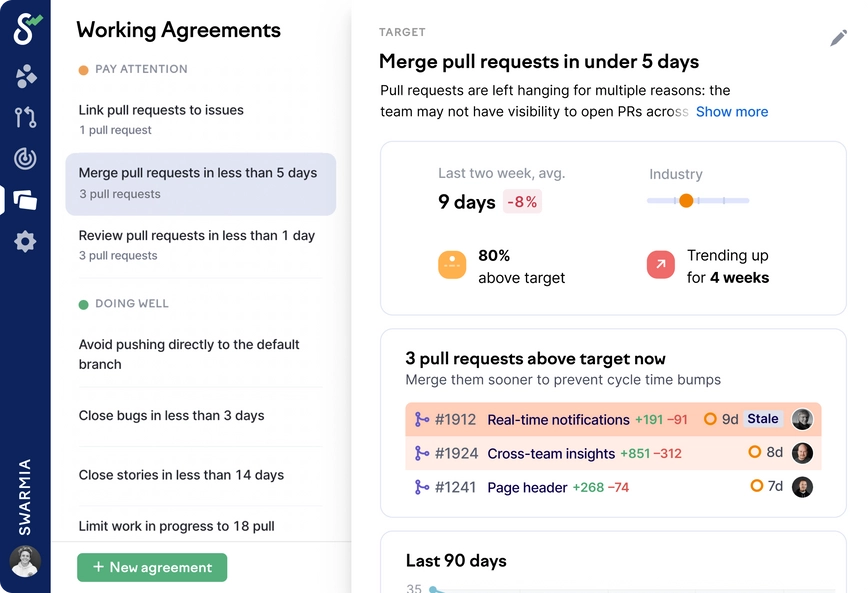
\includegraphics[width=13.5cm]{LaTeX/images/improvement.png}
        \caption{Working Agreements in Swarmia}
        \label{fig:WorkingAgreements}
    \end{center}
\end{figure}

\section{Data}

The data collected by Swarmia includes, but is not limited to, pull requests, issues, and failed deployments. Furthermore, Swarmia has read-only access to the source code, which is used to estimate the complexity of the change in question. Swarmia never stores client code but instead calculates the size of the change bundle and stores it in a separate database. 

Processing of the data is done in Google's BigQuery data warehouse service. Most of the information needed is already collected at Swarmia for business intelligence purposes but needs to be structured in a suitable format. The data flow is shown in Figure \ref{fig:dataFlow}.

\begin{figure}[ht]
\centering
\begin{tikzpicture}[
    every node/.style={align=center, minimum height=1em, minimum width=1cm,node distance=0.7cm},
]

%Nodes
\node[entity]      (teamswa)        {active teams with WA adoption};
\node[entity]      (teams)          [above=of teamswa] {team basic info};
\node[entity]      (snapshots)       [left=of teams] {team snapshots};
\node[entity]       (mau)           [right=of teams] {MAU};
\node[entity]      (ctwa)       [below=of teamswa] {cycle times with WA adoption};
\node[entity]      (cycletimes)       [left=of ctwa]     {cycle times};
\node[entity]      (adoption)       [left=of snapshots] {WA adoption};
\node[entity, fill=gray!20]       (lm)        [below=of ctwa] {linear model input data};

%Lines
\draw[->] (cycletimes.east) -- (ctwa.west);
\draw[->] (ctwa.south) -- (lm.north);
\draw[->] (teamswa.south) -- (ctwa.north);
\draw[->] (teams.south) -- (teamswa.north);
\draw[->] (snapshots.south) -- (teamswa.north);
\draw[->] (mau.south) -- (teamswa.north);
\draw[->] (adoption.south) -- (teamswa.north);

\end{tikzpicture}
\caption{Data flow in BigQuery}
\label{fig:dataFlow}
\end{figure}


\newcommand*\rot{\rotatebox{90}}
\begin{table}[ht]
\begin{center}
\begin{tabular}{|c|c|c|c|c|c|c|c|c|c|c|c|c|c|} 
\hline

No & A & B & C & D & E & F & G & H & ct\_days & slack\_users & daily\_digest \\ [0.5ex]
\hline\hline

1 & 0 & 1 & 0 & 0 & 0 & 0 & 1 & 0 & 1.3 & 2 & 0 \\
2 & 0 & 1 & 0 & 0 & 0 & 0 & 0 & 1 & 0.00031 & 0 & 0 \\ 
3 & 1 & 0 & 1 & 0 & 0 & 0 & 1 & 0 & -0.46 & 4 & 1 \\
4 & 0 & 0 & 0 & 0 & 0 & 0 & 0 & 1 & -0.058 & 5 & 1 \\
5 & 0 & 1 & 1 & 0 & 1 & 1 & 1 & 1 & -1.8 & null & 1 \\

\hline
\end{tabular}
\caption{Sample rows of lm\_data}
\label{tab:dataExample}
\end{center}
\end{table}


For this study, weekly aggregates of team metrics were exported from the Swarmia application backend to BigQuery. This data set is called "cycle times" in Figure \ref{fig:dataFlow}. These metrics were merged with basic team information, working agreement usage, and team member activity. Finally, team identifiers and timestamps were removed so the data points would be independent. A resulting data sample is displayed in Table \ref{tab:dataExample}.

\section{Research questions}

The main research question of this thesis is to look into how teams use Working Agreements: which share of Swarmia teams use each agreement and how these teams have configured their Working Agreements setup. 

The second research question is to determine if Working Agreements can influence cycle times in software development teams. The hypothesis based on previous research is that as Working Agreements promote methods that accelerate software development, they should directly impact the team's performance. We will look into the Working Agreement composition in different teams and determine which agreements impact the teams' cycle times most. 

\section{Approach}

To answer RQ1, data from Swarmia is used to determine how many of the teams have enabled which Working Agreements. Furthermore, we look into how many Working Agreements teams usually use and what goals they have configured for the WAs. For example, WIP limit agreements require teams to specify a threshold for open items. Lastly, team characteristics, such as team size, and their connection to the Working Agreements setup, are analyzed.

Data from all teams using the Working Agreements feature is collected and analyzed to help answer RQ2. Historical activity data is pulled from the teams' source control repositories from 1 July 2020 to 31 July 2022. The data is aggregated weekly for 24 months: some teams have been clients for longer than two years, and some for a shorter amount. The variability of the data collection period should be acceptable, as averages are used, and the period length is not a variable in the analysis.

\begin{figure}[ht]
    \begin{center}
        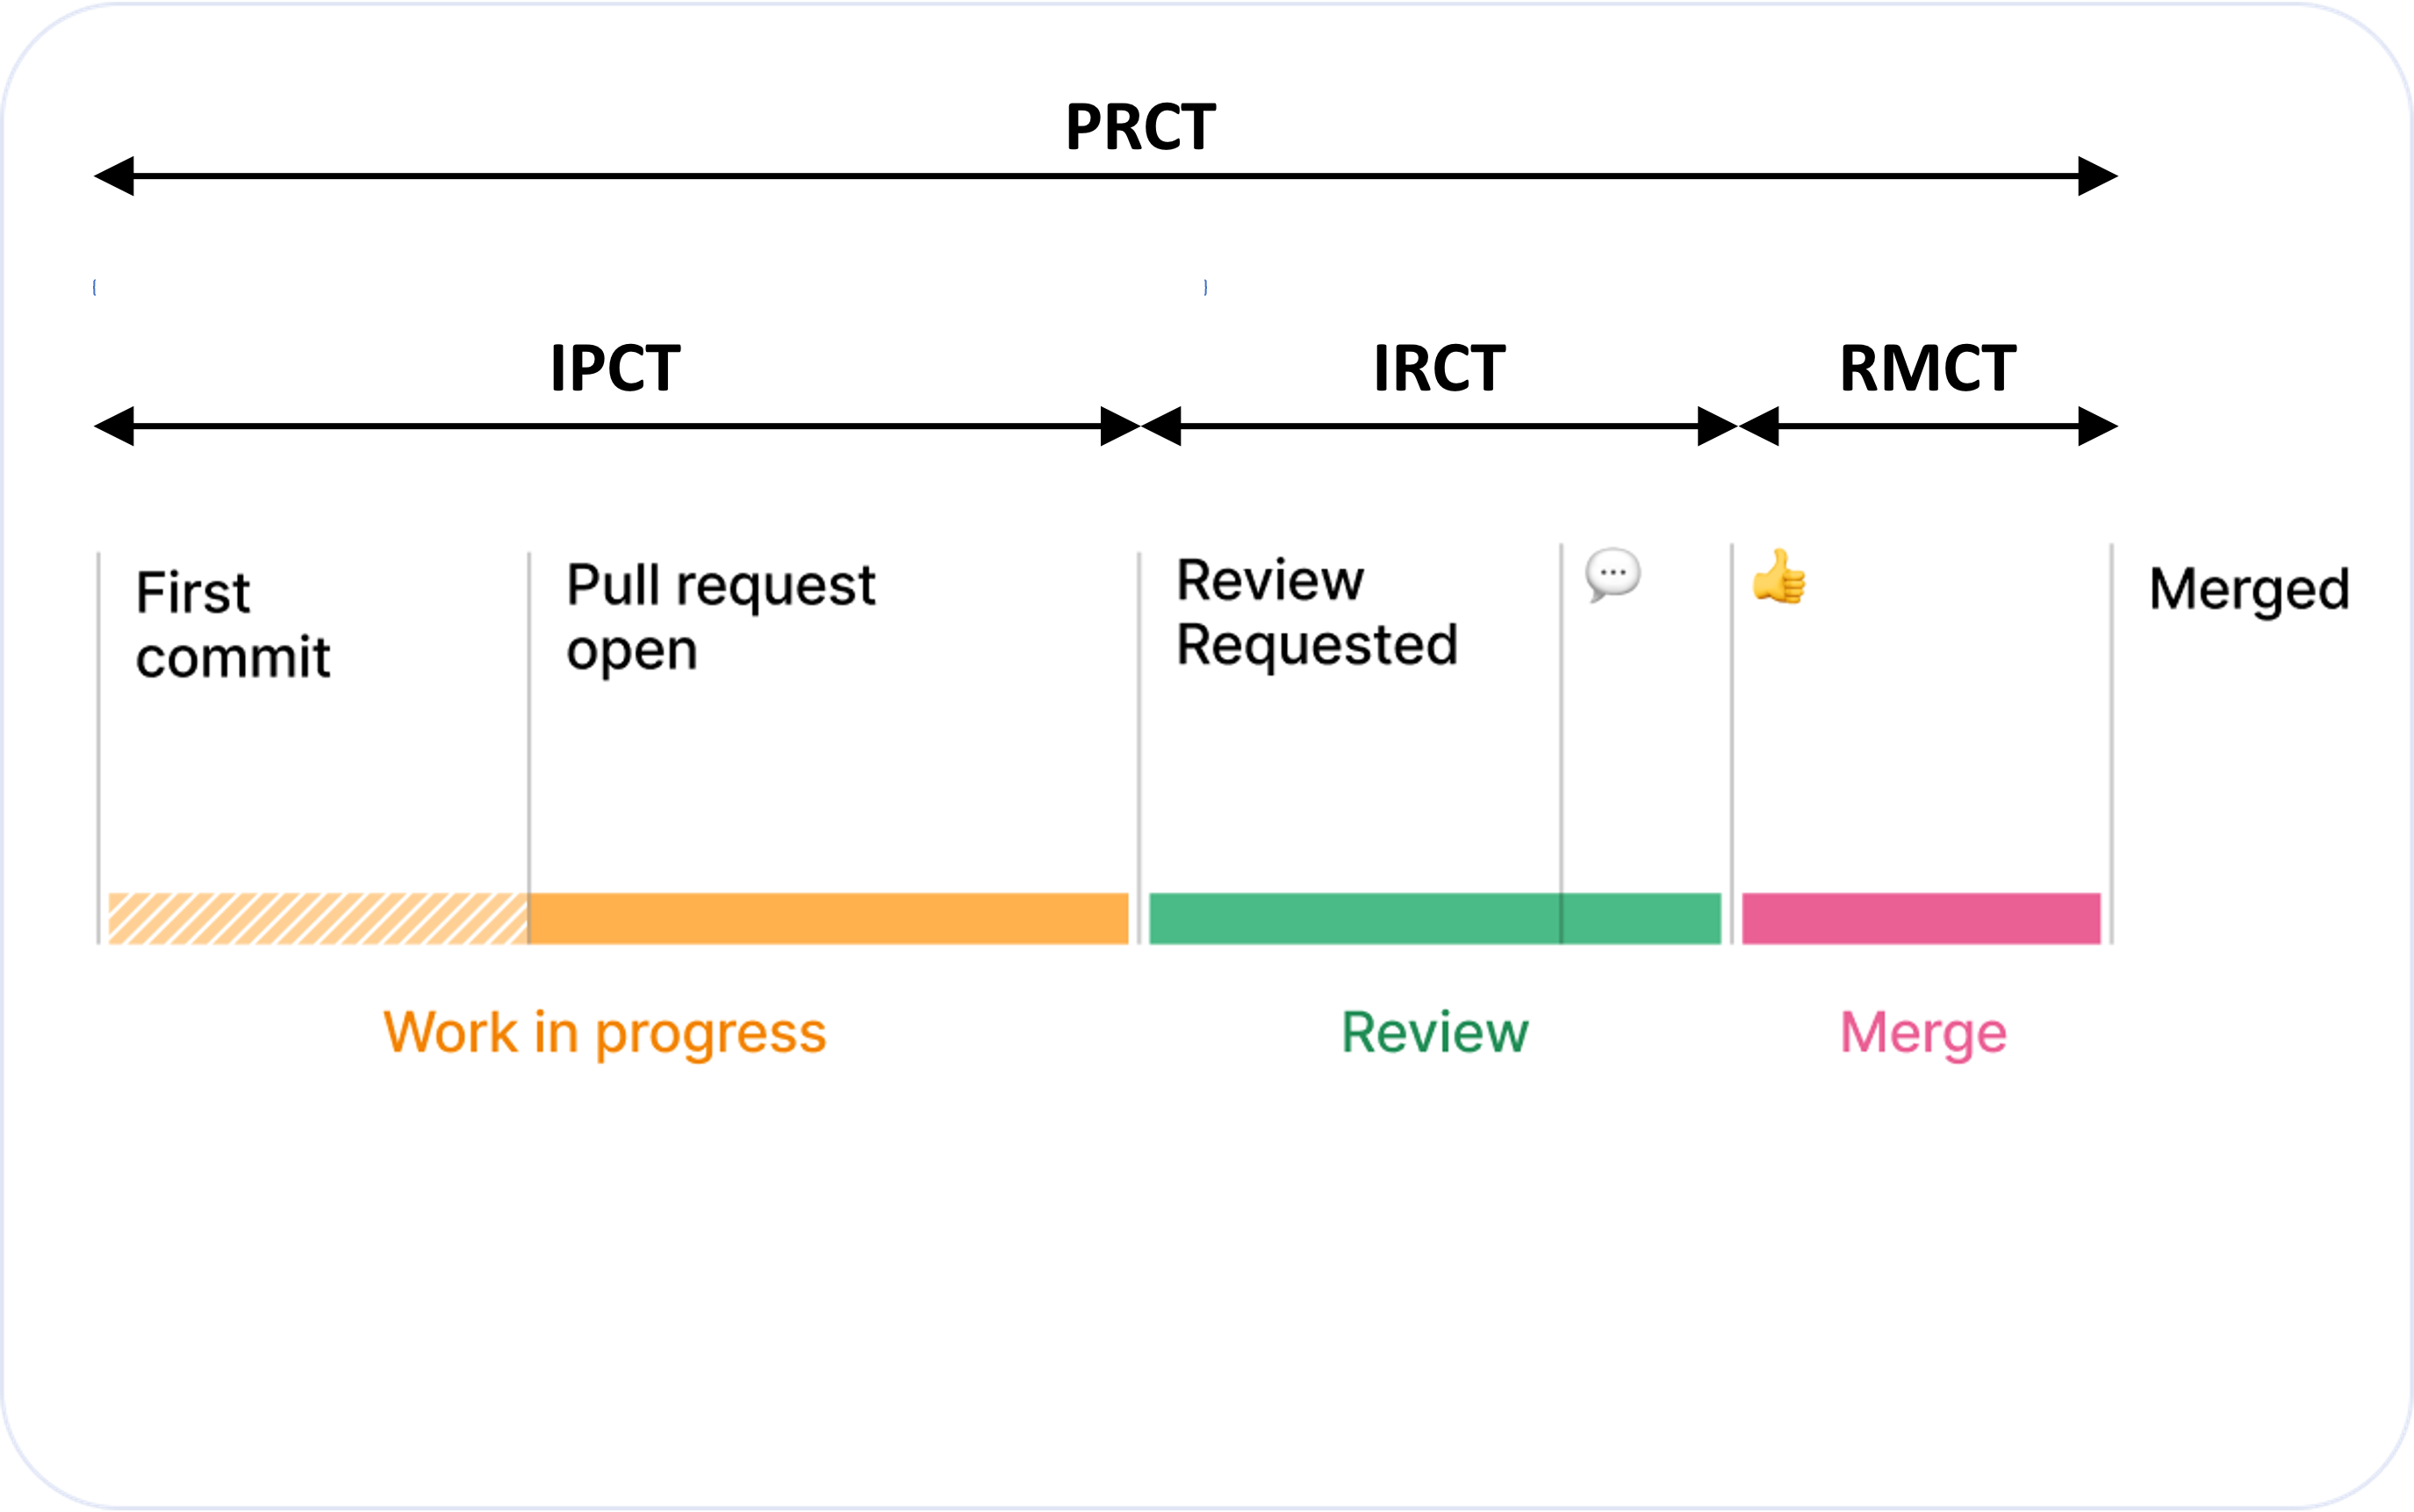
\includegraphics[width=13.5cm]{LaTeX/images/cts-defined-arrows.png}
        \caption{Cycle time definitions}
        \label{fig:ctsArrows}
    \end{center}
\end{figure}

The key metric used in the analysis is the Pull Request Cycle Time (PRCT). Additionally, we look into the sub-parts of PRCT: In Progress Cycle Time (IPCT), In Review Cycle Time (IRCT), and Ready to Merge Cycle Time (RMCT). The span of these metrics in relation sto each other is shown in Figure \ref{fig:ctsArrows}. 

Even though Swarmia exports data from issue trackers, these data sources were left out of the analysis based on the scope of the thesis. The analysis is done in BigQuery in line with Swarmia's privacy policy. In addition to a standard SQL query engine, BigQuery offers advanced data analysis capabilities. For this thesis, the inbuilt linear regression feature was utilized. Figure \ref{fig:dataFlow} presents the data flow before building the regression model. 

We look at the relationship between the independent and dependent variables in linear regression. The dependent variable is the one that, as a hypothesis, depends on the values of the independent variables. Respectively, the independent variables are the configuration of Working Agreements, team member metrics, and Slack notification settings. 

\definecolor{cor-very-weak}{HTML}{BBBBBB}
\definecolor{cor-weak}{HTML}{EEBD84}
\definecolor{cor-moderate}{HTML}{F47461}
\definecolor{cor-strong}{HTML}{F47461}
\definecolor{cor-very-strong}{HTML}{8B0000}

\begin{table}[ht]
\centering
\resizebox{\columnwidth}{!}{
\begin{tabular}{c c c c c c c c c c c c c}

& A & B & C & D & E & F & G & H & ga & sw & sl & dd\\ \hline
A & \textcolor{cor-very-strong}{1.0} & \textcolor{cor-moderate}{0.49} & \textcolor{cor-weak}{0.28} & \textcolor{cor-very-weak}{0.16} & \textcolor{cor-weak}{0.29} & \textcolor{cor-very-weak}{0.15} & \textcolor{cor-moderate}{0.42} & \textcolor{cor-weak}{0.24} & \textcolor{cor-very-weak}{-0.09} & \textcolor{cor-very-weak}{-0.04} & \textcolor{cor-very-weak}{-0.03} & \textcolor{cor-weak}{0.2}\\ \hline
B &  & \textcolor{cor-very-strong}{1.0} & \textcolor{cor-weak}{0.23} & \textcolor{cor-very-weak}{0.18} & \textcolor{cor-weak}{0.32} & \textcolor{cor-weak}{0.31} & \textcolor{cor-strong}{0.64} & \textcolor{cor-weak}{0.39} & \textcolor{cor-very-weak}{-0.07} & \textcolor{cor-very-weak}{0.02} & \textcolor{cor-very-weak}{0.06} & \textcolor{cor-weak}{0.23}\\ \hline
C &  &  & \textcolor{cor-very-strong}{1.0} & \textcolor{cor-weak}{0.25} & \textcolor{cor-weak}{0.26} & \textcolor{cor-very-weak}{0.16} & \textcolor{cor-weak}{0.24} & \textcolor{cor-weak}{0.35} & \textcolor{cor-very-weak}{-0.1} & \textcolor{cor-very-weak}{0.0} & \textcolor{cor-very-weak}{-0.06} & \textcolor{cor-very-weak}{0.09}\\ \hline
D &  &  &  & \textcolor{cor-very-strong}{1.0} & \textcolor{cor-weak}{0.3} & \textcolor{cor-weak}{0.25} & \textcolor{cor-very-weak}{0.15} & \textcolor{cor-weak}{0.3} & \textcolor{cor-very-weak}{0.03} & \textcolor{cor-very-weak}{0.09} & \textcolor{cor-very-weak}{0.0} & \textcolor{cor-very-weak}{0.03}\\ \hline
E &  &  &  &  & \textcolor{cor-very-strong}{1.0} & \textcolor{cor-moderate}{0.58} & \textcolor{cor-weak}{0.28} & \textcolor{cor-moderate}{0.43} & \textcolor{cor-very-weak}{-0.09} & \textcolor{cor-very-weak}{0.01} & \textcolor{cor-very-weak}{-0.02} & \textcolor{cor-very-weak}{0.15}\\ \hline
F &  &  &  &  &  & \textcolor{cor-very-strong}{1.0} & \textcolor{cor-weak}{0.32} & \textcolor{cor-weak}{0.34} & \textcolor{cor-very-weak}{-0.03} & \textcolor{cor-very-weak}{0.08} & \textcolor{cor-very-weak}{0.05} & \textcolor{cor-very-weak}{0.19}\\ \hline
G &  &  &  &  &  &  & \textcolor{cor-very-strong}{1.0} & \textcolor{cor-weak}{0.3} & \textcolor{cor-very-weak}{-0.01} & \textcolor{cor-very-weak}{0.03} & \textcolor{cor-very-weak}{0.08} & \textcolor{cor-weak}{0.32}\\ \hline
H &  &  &  &  &  &  &  & \textcolor{cor-very-strong}{1.0} & \textcolor{cor-very-weak}{-0.09} & \textcolor{cor-very-weak}{0.0} & \textcolor{cor-very-weak}{-0.01} & \textcolor{cor-very-weak}{0.1}\\ \hline
ga &  &  &  &  &  &  &  &  & \textcolor{cor-very-strong}{1.0} & \textcolor{cor-strong}{0.79} & \textcolor{cor-strong}{0.78} & \textcolor{cor-very-weak}{-0.18}\\ \hline
sw &  &  &  &  &  &  &  &  &  & \textcolor{cor-very-strong}{1.0} & \textcolor{cor-very-strong}{0.84} & \textcolor{cor-very-weak}{-0.07}\\ \hline
sl &  &  &  &  &  &  &  &  &  &  & \textcolor{cor-very-strong}{1.0} & \textcolor{cor-very-weak}{-0.01}\\ \hline
dd &  &  &  &  &  &  &  &  &  &  &  & \textcolor{cor-very-strong}{1.0}\\ \hline

\end{tabular}
}

\caption{Correlation matrix. The stronger the correlation, the darker the color. ga=github\_authors, sw=swarmia\_users, sl=slack\_users, dd=daily\_digest}
\label{tab:correlationMatrix}
\end{table}

Pearson correlation coefficient for independent variables is calculated in Table \ref{tab:correlationMatrix} to ensure the data is compatible with linear regression analysis: two variables should not correlate for the model to work as expected. The most considerable correlation encountered is the of slack\_users and swarmia\_users with a value of 0.84. The pairs with high correlation deal with the same themes, for example, WAs related to pull requests. Even though some of the WAs correlate, the data can be used for the model with slight modifications: github\_authors and swarmia\_users were dropped to include only the team member metric, slack\_users. 

\begin{samepage}

Linear regression can be formulated as follows:
\begin{equation}
Y = \beta_0 + \beta_i X_i + \beta_{i+1} X_{i+1} + \ldots + \beta_n X_n + \epsilon
\end{equation}

where
\begin{description}
\item $Y$ is dependent variable
\item $\beta_0$ is constant coefficient (intercept)
\item $\beta_i$ is slope for $X_i$
\item $X_i$ is independent variable
\item $\epsilon$ is error
\end{description}

\end{samepage}

The training data is passed to linear regression in a form presented in Table \ref{tab:trainingDataStructure}. The data has gone through two significant modifications to suit linear regression. First, we calculated average cycle times for each team before they enabled any Working Agreements. This average is then subtracted from each data point's cycle time to achieve a normalized data set: the aim is to diminish the differences between teams to achieve comparable cycle times. Secondly, WA activation dates are mapped to Boolean values for each row: the value is zero if WA has not been activated yet and one if it has.

\begin{table}
\begin{center}
\begin{tabularx}{\textwidth}{ |l|X| } 
\hline
parameter & description \\ [0.5ex] 
\hline\hline
wip\_pull\_requests & WA status \\
max\_pull\_request\_age & WA status \\
no\_direct\_pushes\_to\_main\_branch & WA status \\
min\_issue\_contributors  & WA status \\
wip\_issues & WA status \\
max\_issue\_age  & WA status \\
max\_pull\_request\_review\_time  & WA status \\
pull\_request\_linking  & WA status \\
ct\_days  & normalized cycle time in days \\
github\_authors & Pull request authors \\
swarmia\_users & MAU in Swarmia team \\
slack\_users & Swarmia users with Slack notifications \\
daily\_digest & team's Slack daily digest status \\
\hline
\end{tabularx}
\caption{Linear regression training data structure}
\label{tab:trainingDataStructure}
\end{center}
\end{table}




At the beginning of the analysis, three team member-related metrics were included: github\_authors, swarmia\_users, and slack\_users. The amount of Swarmia users did not have statistical significance and strongly correlated with github\_authors with a correlation of $0.79$. In the end, out of the three metrics, only slack\_users was retained in the final model.

The model was also run with PRCT components: IPCT, IRCT, and RMCT. The aim was to investigate which part of the process the independent variables mainly influenced. Only modeling against In Progress Cycle Time produced results with statistical significance. Finally, the targets set for max\_pull\_request\_review\_time and max\_pull\_request\_age were studied with dedicated models. These target models use a Boolean independent variable, calculated with the formula $cycle\_time<target$. The dependent variables included are daily\_digest, slack\_users, days\_in\_use: the days the WA has been in use, and target\_days: the set target for the given WA. 

The threshold value $\alpha$ selected for the study diverts from the standard convention of $\alpha=0.05$. Instead, results with a p-value of $p<0.10$ are considered as having statistical significance against the null hypothesis. Furthermore, results with a p-value of $p<0.05$ and $p<0.01$ were given additional noteworthiness. These three categories of significance are denoted with asterisks in figures and tables. 

In the study, the conclusions are not solely based on p-value: it is instead utilized as a variable that supports the broader analysis. Especially weights of the independent variables are considered crucial when interpreting the results. 



\chapter{Discussion}
\section{Future work}
\section{Conclusion}



% Load the bibliographic references
% ------------------------------------------------------------------
% You can use several .bib files:
% \bibliography{thesis_sources,ietf_sources}
\bibliography{LaTeX/references}

\appendix
%\input{9appendix.tex}

\end{document}